\subsubsection{Simple convection in a spherical 3d shell}
\label{sec:shell-simple-3d}

The setup from the previous section can of course be extended to 3d shell
geometries as well -- though at significant computational cost. In fact, the
number of modifications necessary is relatively small, as we will discuss below.
To show an example up front, a picture of the temperature field one gets from
such a simulation is shown in Fig.~\ref{fig:simple-shell-3d}. The
corresponding movie can be found at \url{http://youtu.be/j63MkEc0RRw}.

\begin{figure}[tb]
\centering
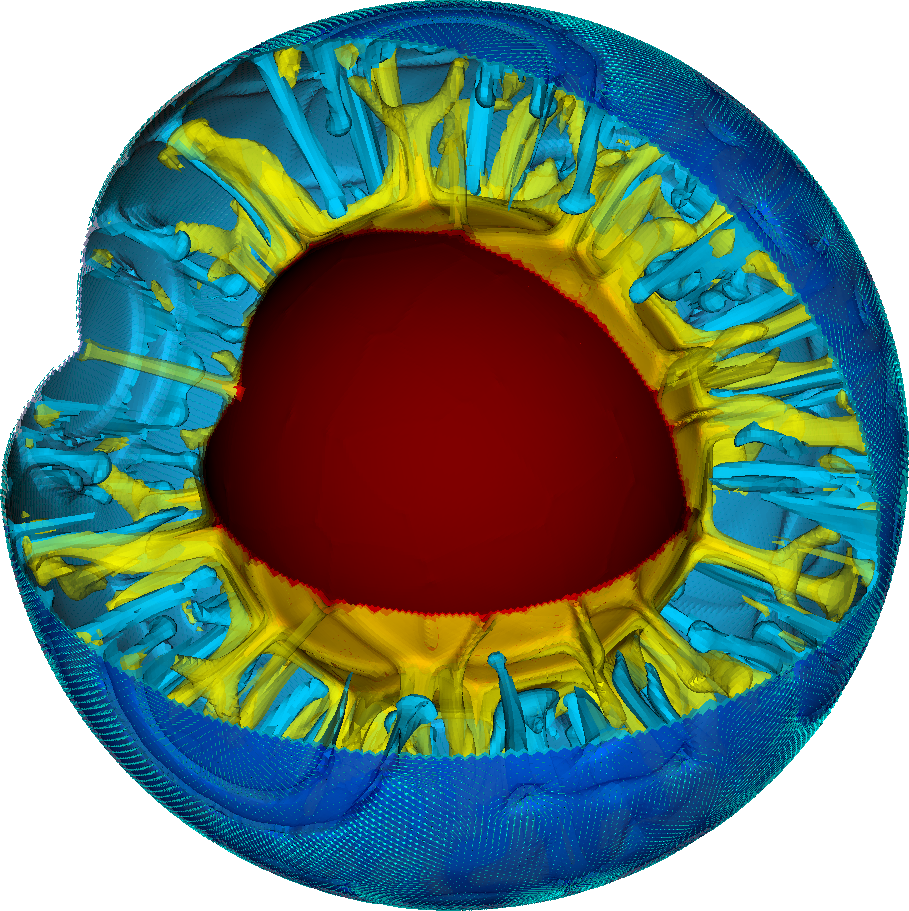
\includegraphics[width=0.7\textwidth]{cookbooks/shell_simple_3d/doc/x-movie0700.png}
\caption{\it Convection in a spherical shell: Snapshot of
isosurfaces of the temperature field at time $t\approx \num{1.06e9}$ years
with a quarter of the geometry cut away. The surface shows
vectors indicating the flow velocity and direction.}
\label{fig:simple-shell-3d}
\end{figure}

\paragraph{The input file.}
Compared to the input file discussed in the previous section, the number of
changes is relatively small. However, when taking into account the various
discussions about which parts of the model were or were not realistic, they go
throughout the input file, so we reproduce it here in its entirety, interspersed
with comments (the full input file can also be found in
\url{cookbooks/shell_simple_3d/shell_simple_3d.prm}). Let us start from the top where everything
looks the same except that we set the dimension to 3:

\lstinputlisting[language=prmfile]{cookbooks/shell_simple_3d/doc/part1.part.prm.out}

The next section concerns the geometry. The geometry model remains unchanged at
``spherical shell'' but we omit the opening angle of 90 degrees as we would like
to get a complete spherical shell. Such a shell of course also only has two
boundaries (the inner one has indicator zero, the outer one indicator one) and
consequently these are the only ones we need to list in the ``Boundary velocity model''
section:

\lstinputlisting[language=prmfile]{cookbooks/shell_simple_3d/doc/part2.part.prm.out}

Next, since we convinced ourselves that the temperature range from 973 to 4273
was too large given that we do not take into account adiabatic effects in this
model, we reduce the temperature at the inner edge of the mantle to 1973. One
can think of this as an approximation to the real temperature there minus the
amount of adiabatic heating material would experience as it is transported from
the surface to the core-mantle boundary. This is, in effect, the temperature
difference that drives the convection (because a completely adiabatic
temperature profile is stable despite the fact that it is much hotter at the
core mantle boundary than at the surface). What the real value for this
temperature difference is, is unclear from current research, but it is thought
to be around 1000 Kelvin, so let us choose these values.

\lstinputlisting[language=prmfile]{cookbooks/shell_simple_3d/doc/part3.part.prm.out}

The second component to this is that we found that without adiabatic effects, an
initial temperature profile that decreases the temperature from the inner to the
outer boundary makes no sense. Rather, we expected a more or less constant
temperature with boundary layers at both ends. We could describe such an initial
temperature field, but since any initial temperature is mostly arbitrary anyway,
we opt to just assume a constant temperature in the middle between the inner and
outer temperature boundary values and let the simulation find the exact shape of
the boundary layers itself:

\lstinputlisting[language=prmfile]{cookbooks/shell_simple_3d/doc/part4.part.prm.out}

As before, we need to determine how many mesh refinement steps we want. In 3d,
it is simply not possible to have as much mesh refinement as in 2d, so we choose
the following values that lead to meshes that have, after an initial transitory
phase, between 1.5 and 2.2 million cells and 50--75 million unknowns:

\lstinputlisting[language=prmfile]{cookbooks/shell_simple_3d/doc/amr.part.prm.out}

Second to last, we specify what we want \aspect{} to do with the solutions it
computes. Here, we compute the same statistics as before, and we again generate
graphical output every million years. Computations of this size typically run
with ~1000 MPI processes, and it is not efficient to let every one of them write
their own file to disk every time we generate graphical output; rather, we group
all of these into a single file to keep file systems reasonably happy. Likewise,
to accommodate the large amount of data, we output depth averaged fields in VTU
format since it is easier to visualize:

\lstinputlisting[language=prmfile]{cookbooks/shell_simple_3d/doc/postprocess.part.prm.out}

Finally, we realize that when we run very large parallel computations, nodes go
down or the scheduler aborts programs because they ran out of time. With
computations this big, we cannot afford to just lose the results, so we
checkpoint the computations every 50 time steps and can then resume it at the
last saved state if necessary (see Section~\ref{sec:checkpoint-restart}):

\lstinputlisting[language=prmfile]{cookbooks/shell_simple_3d/doc/checkpoint.part.prm.out}




\paragraph{Evaluation.}
Just as in the 2d case above, there are still many things that are wrong from a
physical perspective in this setup, notably the no-slip boundary conditions at
the bottom and of course the simplistic material model with its fixed viscosity
and its neglect for adiabatic heating and compressibility.
But there are also a number of things that are already order of magnitude
correct here.

For example, if we look at the heat flux this model produces, we find that the
convection here produces approximately the correct number. Wikipedia's article
on \href{http://en.wikipedia.org/wiki/Earth's_internal_heat_budget}{Earth's
internal heat budget}%
\footnote{Not necessarily the most scientific source, but easily
accessible and typically about right in terms of numbers. The numbers stated
here are those listed on Wikipedia at the time this section was written in
March 2014.}
states that the overall heat flux through the Earth surface is about $\num{47e12}$ W (i.e., 47 terawatts) of which an estimated 12--30 TW are primordial
heat released from cooling the Earth and 15--41 TW from radiogenic heating.%
\footnote{As a point of reference, for the mantle an often used number for the
release of heat due to radioactive decay is $\num{7.4e-12}$ W/kg. Taking a
density of $3300\; \si{kg}/\si{m}^3$ and a volume of $10^{12}\; \si{m}^3$
would yield roughly $\num{2.4e13}$ W of heat produced. This back of the
envelope calculation lies within the uncertain range stated above.}
Our model does not include radiogenic heating (though \aspect{} has a number of
\texttt{Heating models} to switch this on, see
Section~\ref{parameters:Heating_20model}) but we can compare what the model
gives us in terms of heat flux through the inner and outer boundaries of our
shell geometry. This is shown in the left panel of
Fig.~\ref{fig:shell-simple-3d-eval} where we plot the heat flux through
boundaries zero and one, corresponding to the core-mantle boundary and Earth's
surface. \aspect{} always computes heat fluxes in outward direction, so the flux
through boundary zero will be negative, indicating the we have a net flux
\textit{into} the mantle as expected. The figure indicates that after some
initial jitters, heat flux from the core to the mantle stabilizes at around 4.5
TW and that through the surface at around 10 TW, the difference of 5.5 TW
resulting from the overall cooling of the mantle. While we cannot expect our model to be
quantitatively correct, this can be compared with estimated heat fluxes of 5--15
TW for the core-mantle boundary, and an estimated heat loss due to cooling of
the mantle of 7--15 TW (values again taken from Wikipedia).

\begin{figure}
  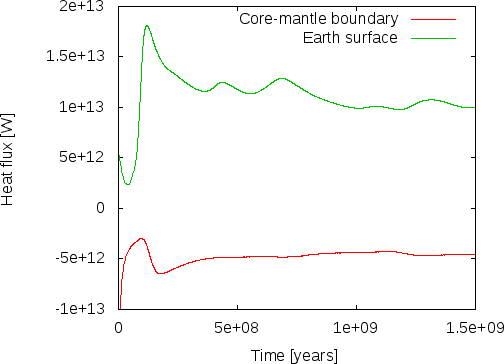
\includegraphics[width=0.48\textwidth]{cookbooks/shell_simple_3d/doc/heatflux.png}
  \hfill
  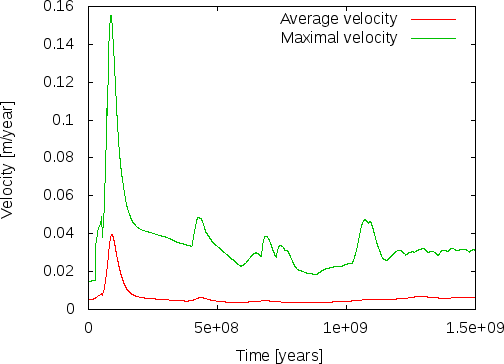
\includegraphics[width=0.48\textwidth]{cookbooks/shell_simple_3d/doc/velocities.png}
  \caption{\it Evaluating the 3d spherical shell model. Left: Outward heat
  fluxes through the inner and outer boundaries of the shell. Right: Average
  and maximal velocities in the mantle.}
  \label{fig:shell-simple-3d-eval}
\end{figure}

A second measure of whether these results make sense is to compare velocities in
the mantle with what is known from observations. As shown in the right panel of
Fig.~\ref{fig:shell-simple-3d-eval}, the maximal velocities settle to values on
the order of 3 cm/year (each of the peaks in the line for the maximal velocity
corresponds to a particularly large plume rising or falling). This is, again, at
least not very far from what we know to be correct and we should expect that
with a more elaborate material model we should be able to get even closer to
reality.
